% My own macros
\newcommand{\ensuretext}[1]{\ensuremath{\text{#1}}}
\def\ie{\ensuretext{\textit{i.e.,\xspace}}}
\def\eg{\ensuretext{\textit{e.g.,\xspace}}}

\newcommand{\uder}[2]{\frac{\partial #1}{\partial #2}}
\newcommand{\C}{\ensuremath{\mathbb{C}}}
\newcommand{\CP}{\ensuremath{\mathbb{CP}}}
\newcommand{\GL}[1]{\ensuremath{\mathrm{GL}(#1)}}
\newcommand{\SL}[1]{\ensuremath{\mathrm{SL}(#1)}}
\newcommand{\Q}{\ensuremath{\mathbb{Q}}}
\newcommand{\R}{\ensuremath{\mathbb{R}}}
\newcommand{\RP}{\ensuremath{\mathbb{RP}}}
\newcommand{\Z}{\ensuremath{\mathbb{Z}}}
\newcommand{\med}{\ensuremath{\mathop{\mathrm{med}}}}
\newcommand{\uPr}{\ensuremath{\mathop{\mathrm{Pr}}}}
\newcommand{\uE}{\ensuremath{\mathrm{E}}}
\newcommand{\ucov}[2]{\ensuremath{\mathop{\mathrm{cov}}\left(#1 ,\, #2\right)}}
\newcommand{\ucor}[2]{\ensuremath{\mathop{\mathrm{corr}}\left(#1 ,\, #2\right)}}
\newcommand{\ucorr}[2]{\ensuremath{\mathop{\mathrm{corr}}\left(#1 ,\, #2\right)}}
\newcommand{\uvar}{\ensuremath{\mathop{\mathrm{var}}}}
\newcommand{\ud}{\ensuremath{\mathrm{d}}}
\newcommand{\uProj}{\ensuremath{\mathop{\mathrm{Proj}}}}
\newcommand{\uimply}{\ensuremath{\;\Longrightarrow\;}}
\newcommand{\uequiv}{\ensuremath{\;\Longleftrightarrow\;}}
\newcommand{\uforall}{\textrm{ for all }}
\newcommand{\us}[1]{\ensuremath{\mathrm{Sym}(#1)}}
\newcommand{\uo}[2]{\mathrm{Orb}_{#1}(#2)}
\newcommand{\ustab}[1]{\mathrm{Stab}(#1)}
\newcommand{\uinner}[2]{\ensuremath{\langle #1 ,\; #2 \rangle}}
\newcounter{myN}
\newcommand{\urepeat}[2]{%
  \setcounter{myN}{0}
  \whiledo{\value{myN} < #1}{%
    \stepcounter{myN}#2}}
\newcommand{\uvec}[2][n]{\ensuremath{#2_1, \cdots, #2_{#1}}}
\newcommand{\umark}[1]{\marginpar{%
    \vskip-\baselineskip %raise the marginpar a bit
    \raggedright\footnotesize
    \itshape\hrule\smallskip#1\par\smallskip\hrule}}





%%%%%%%%%%%%%% Front matters

\begin{frame}
  \titlepage
\end{frame}

\begin{frame}
  \frametitle{Outline}
  \tableofcontents
  % You might wish to add the option [pausesections]
\end{frame}

%%%%%%%%%%%%% Main text

\section{Probability distributions}

\begin{frame}
  \frametitle{Random variables and probability}
  \begin{itemize}
  \item A brief overview of random variables. \item $X(\omega) : \Omega
    \to \R$.
  \item Binary (Bernoulli), a special case of discrete r.v.
  \item Discrete (binomial, Poisson, negative binomial, ...)
  \item Continuous (normal, chi-squared, logistic, ...)
  \item Notion of independence/dependence; $i.i.d.$; what constitutes a
    \textbf{sample}?
  \end{itemize}
\end{frame}

\begin{frame}[fragile]
  \frametitle{Built-in probability functions}
\begin{knitrout}\footnotesize
\definecolor{shadecolor}{rgb}{0.969, 0.969, 0.969}\color{fgcolor}\begin{kframe}
\begin{alltt}
\hlstd{x1} \hlkwb{<-} \hlkwd{rgeom}\hlstd{(}\hlnum{10}\hlstd{,} \hlnum{1}\hlopt{/}\hlnum{3}\hlstd{)}       \hlcom{#geometric r.v., discrete.}
\hlstd{x2} \hlkwb{<-} \hlkwd{rbinom}\hlstd{(}\hlnum{10}\hlstd{,} \hlnum{1}\hlstd{,} \hlnum{1}\hlopt{/}\hlnum{2}\hlstd{)}   \hlcom{#standard Bernoulli (fair coin)}
\hlstd{x3} \hlkwb{<-} \hlkwd{rnorm}\hlstd{(}\hlnum{10}\hlstd{)}            \hlcom{#standard normal (mean=0, sd=1)}
\hlstd{x4} \hlkwb{<-} \hlkwd{rnorm}\hlstd{(}\hlnum{100}\hlstd{,} \hlnum{5}\hlstd{,} \hlnum{2}\hlstd{)}    \hlcom{#mean=5, sd=2.}
\hlkwd{mean}\hlstd{(x4);} \hlkwd{sd}\hlstd{(x4)}           \hlcom{#convergence}
\end{alltt}
\begin{verbatim}
## [1] 5.081998
## [1] 2.014264
\end{verbatim}
\end{kframe}
\end{knitrout}

\end{frame}

\begin{frame}
  \frametitle{Built-in functions (II)}
  \begin{itemize}
  \item Probability density function, \textit{a.k.a.} \textit{p.d.f.}.
    qDiscrete/continuous.  In R: \texttt{dbinom()}, \texttt{dnorm()},
    \texttt{dchisq()}, etc.
  \item Probability distribution function, \textit{a.k.a.}
    \textit{c.d.f.}. In R: \texttt{p<name>}.
  \item Quantile function. In R: \texttt{q<name>}.
  \end{itemize}
\end{frame}

\begin{frame}[fragile]
  \frametitle{Useful functions}
  \begin{itemize}
  \item \texttt{summary()}, \texttt{fivenum()}, \texttt{stem()}.
  \item \texttt{hist()}, \texttt{density()}, \texttt{rug()},
    \texttt{ecdf()}.
  \item QQ-plots: follow the book example.
  \item Formal normality tests. Useful in residual analysis (goodness of
    fit).
  \end{itemize}
\end{frame}

\begin{frame}[fragile]
\begin{knitrout}\footnotesize
\definecolor{shadecolor}{rgb}{0.969, 0.969, 0.969}\color{fgcolor}\begin{kframe}
\begin{alltt}
\hlstd{grid} \hlkwb{<-} \hlkwd{seq}\hlstd{(}\hlkwd{min}\hlstd{(x4),} \hlkwd{max}\hlstd{(x4),} \hlnum{0.01}\hlstd{)}
\hlkwd{plot}\hlstd{(}\hlkwd{ecdf}\hlstd{(x4))}
\hlkwd{lines}\hlstd{(grid,} \hlkwd{pnorm}\hlstd{(grid,} \hlnum{5}\hlstd{,} \hlnum{2}\hlstd{),} \hlkwc{lty}\hlstd{=}\hlnum{2}\hlstd{,} \hlkwc{col}\hlstd{=}\hlstr{"red"}\hlstd{,} \hlkwc{lwd}\hlstd{=}\hlnum{2}\hlstd{)}
\end{alltt}
\end{kframe}

{\centering 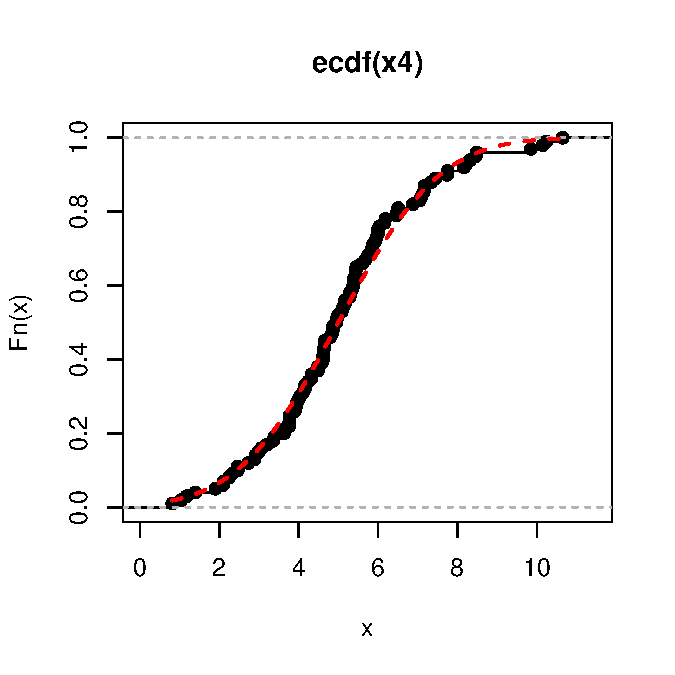
\includegraphics[width=.48\linewidth]{figure/beamer-unnamed-chunk-2-1} 

}



\end{knitrout}
\end{frame}

\section{Group comparisons}

\begin{frame}
  \frametitle{Quick review of hypothesis testing}
  \begin{itemize}
  \item A typical scenario in data analysis is to compare groups.
  \item Even if there is no ``true difference'', sample means
    calculated from different groups will be different due to
    randomness.
  \item Hypothesis testing: $H_{0}$: no group effects versus $H_{1}$:
    group effects are not zero.  $p$-value in a nutshell: How likely
    we'll end up with the observed group difference under $H_{0}$?
  \item Hypothesis testing can be generalized to all correlation
    models, regression models, etc.
  \end{itemize}
\end{frame}


\begin{frame}
  \frametitle{One and two sample tests for continuous data}
  \begin{itemize}
  \item \texttt{t.test()} and variants (one-group v. two group;
    one-sided v. two sided; paired v. unpaired).
  \item \texttt{var.test()}.  The two-fold rule-of-thumb and the Welch
    correction. 
  \item Parametric v. nonparametric test.
  \item \texttt{wilcox.test()} (paired, unpaired).
  \item A few words about \texttt{shapiro.test()}. ``Passing'' this
    test ($p>0.05$) for very small sample size does not mean much.
    Don't do 3 mice versus 3 mice experiments!!
  \item Omnibus test: Kolmogorov-Smirnov test \texttt{ks.test()},
    Cramer-von Mises test (\texttt{cvm.test()}), etc.
  \end{itemize}
\end{frame}

\begin{frame}[fragile]{Two-sample $t$-test and Wilcoxon ranksum test}
\begin{knitrout}\footnotesize
\definecolor{shadecolor}{rgb}{0.969, 0.969, 0.969}\color{fgcolor}\begin{kframe}
\begin{alltt}
\hlstd{X} \hlkwb{<-} \hlkwd{rnorm}\hlstd{(}\hlnum{15}\hlstd{); Y} \hlkwb{<-} \hlkwd{rnorm}\hlstd{(}\hlnum{15}\hlstd{)} \hlopt{+} \hlnum{.8}\hlopt{*}\hlstd{X}
\hlkwd{t.test}\hlstd{(X, Y)}    \hlcom{# Default: two-sided, nonpaired, with correction.}
\hlstd{XY} \hlkwb{<-} \hlkwd{c}\hlstd{(X, Y)}
\hlstd{Grp} \hlkwb{<-} \hlkwd{c}\hlstd{(}\hlkwd{rep}\hlstd{(}\hlstr{"Control"}\hlstd{,} \hlkwd{length}\hlstd{(X)),} \hlkwd{rep}\hlstd{(}\hlstr{"Treatment"}\hlstd{,} \hlkwd{length}\hlstd{(Y)))}
\hlkwd{t.test}\hlstd{(XY}\hlopt{~}\hlstd{Grp)}  \hlcom{#the equivalent formula interface.}
\hlcom{# one-sided test }
\hlkwd{t.test}\hlstd{(XY}\hlopt{~}\hlstd{Grp,} \hlkwc{alternative}\hlstd{=}\hlstr{"less"}\hlstd{)} \hlcom{#less means X<Y}
\hlcom{# Wilcoxon ranksum test is the nonparametric counterpart}
\hlcom{## of two sample t-test}
\hlkwd{wilcox.test}\hlstd{(XY}\hlopt{~}\hlstd{Grp,} \hlkwc{alternative}\hlstd{=}\hlstr{"less"}\hlstd{)}
\end{alltt}
\end{kframe}
\end{knitrout}
\end{frame}

\begin{frame}[fragile]{Two-sample tests (II)}
\begin{knitrout}\footnotesize
\definecolor{shadecolor}{rgb}{0.969, 0.969, 0.969}\color{fgcolor}\begin{kframe}
\begin{alltt}
\hlcom{## Boxplot of the data. It is good to plot the actual data}
\hlcom{## (jittered a little bit) on the boxplot.}
\hlkwd{boxplot}\hlstd{(XY}\hlopt{~}\hlstd{Grp,} \hlkwc{outpch} \hlstd{=} \hlnum{NA}\hlstd{,} \hlkwc{xlab}\hlstd{=}\hlstr{""}\hlstd{,} \hlkwc{ylab}\hlstd{=}\hlstr{"Value"}\hlstd{)}
\hlkwd{stripchart}\hlstd{(XY} \hlopt{~} \hlstd{Grp,} \hlkwc{vertical}\hlstd{=}\hlnum{TRUE}\hlstd{,} \hlkwc{method}\hlstd{=}\hlstr{"jitter"}\hlstd{,} \hlkwc{add}\hlstd{=}\hlnum{TRUE}\hlstd{)}
\end{alltt}
\end{kframe}

{\centering 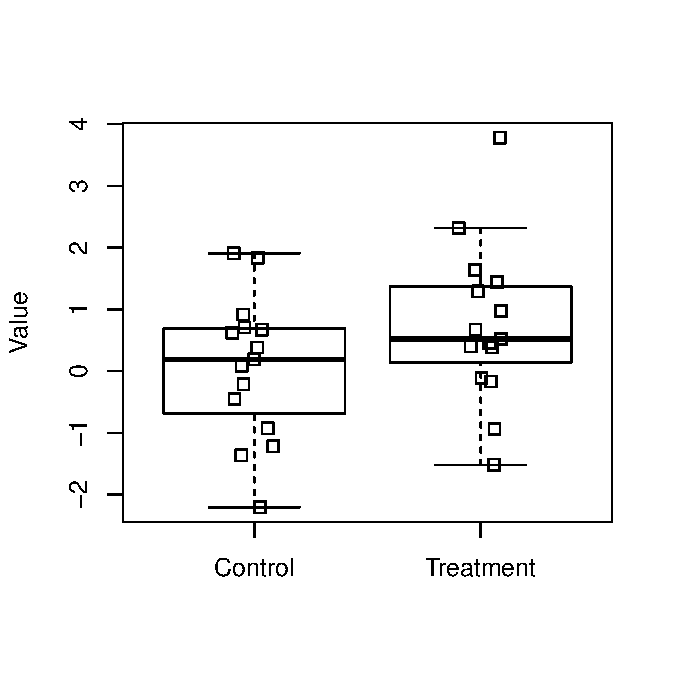
\includegraphics[width=.48\linewidth]{figure/beamer-ttest-plot-1} 

}



\end{knitrout}
\end{frame}

\begin{frame}[fragile]{Paired tests}
\begin{knitrout}\footnotesize
\definecolor{shadecolor}{rgb}{0.969, 0.969, 0.969}\color{fgcolor}\begin{kframe}
\begin{alltt}
\hlcom{## paired, one-sided test (Y greater than X}
\hlstd{Grp2} \hlkwb{<-} \hlkwd{c}\hlstd{(}\hlkwd{rep}\hlstd{(}\hlstr{"Pre"}\hlstd{,} \hlkwd{length}\hlstd{(X)),} \hlkwd{rep}\hlstd{(}\hlstr{"Post"}\hlstd{,} \hlkwd{length}\hlstd{(Y)))}
\hlkwd{t.test}\hlstd{(X, Y,} \hlkwc{paired}\hlstd{=}\hlnum{TRUE}\hlstd{)}
\hlcom{# Wilcoxon signed rank test}
\hlkwd{wilcox.test}\hlstd{(X, Y,} \hlkwc{paired}\hlstd{=}\hlnum{TRUE}\hlstd{)}
\end{alltt}
\end{kframe}
\end{knitrout}
\end{frame}

\begin{frame}[fragile]{Paired test (II)}
\begin{knitrout}\footnotesize
\definecolor{shadecolor}{rgb}{0.969, 0.969, 0.969}\color{fgcolor}\begin{kframe}
\begin{alltt}
\hlkwd{boxplot}\hlstd{(X, Y,} \hlkwc{outpch} \hlstd{=} \hlnum{NA}\hlstd{,} \hlkwc{xlab}\hlstd{=}\hlstr{""}\hlstd{,} \hlkwc{names}\hlstd{=}\hlkwd{c}\hlstd{(}\hlstr{"Pre"}\hlstd{,} \hlstr{"Post"}\hlstd{),}
        \hlkwc{ylab}\hlstd{=}\hlstr{"Value"}\hlstd{,} \hlkwc{col}\hlstd{=}\hlkwd{c}\hlstd{(}\hlstr{"lightgrey"}\hlstd{,} \hlstr{"lightblue"}\hlstd{))}
\hlkwd{stripchart}\hlstd{(}\hlkwd{list}\hlstd{(X, Y),} \hlkwc{vertical}\hlstd{=}\hlnum{TRUE}\hlstd{,} \hlkwc{pch}\hlstd{=}\hlnum{16}\hlstd{,} \hlkwc{add}\hlstd{=}\hlnum{TRUE}\hlstd{)}
\hlcom{## Add line segments to link pre/post together}
\hlstd{s} \hlkwb{<-} \hlkwd{seq}\hlstd{(}\hlkwd{length}\hlstd{(X))}
\hlkwd{segments}\hlstd{(}\hlkwd{rep}\hlstd{(}\hlnum{1}\hlstd{,}\hlkwd{length}\hlstd{(X))[s],X[s],}\hlkwd{rep}\hlstd{(}\hlnum{2}\hlstd{,}\hlkwd{length}\hlstd{(X))[s],Y[s])}
\end{alltt}
\end{kframe}

{\centering 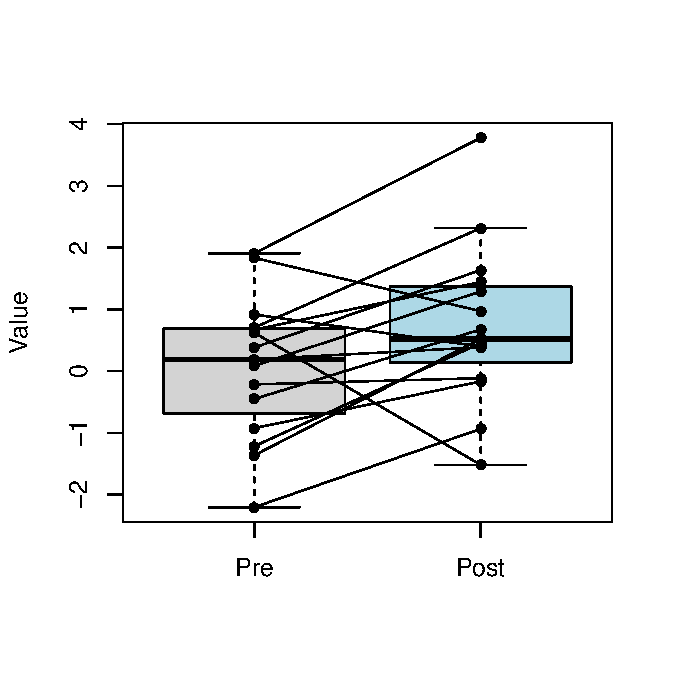
\includegraphics[width=.48\linewidth]{figure/beamer-paired-t-plot-1} 

}



\end{knitrout}
\end{frame}


\section{Linear models and ANOVA}
\label{sec:linear-models}

\begin{frame}{Linear Regression}
  \begin{itemize}
  \item Linear regression is the most popular way to model
    \emph{linear} relationship between covariates ($\mathbf{X}$) and
    continuous responses ($\mathbf{Y}$).
    \begin{equation}
      \label{eq:lin-mod}
      \mathbf{Y} = \mathbf{X} \bm{\beta} + \bm{\epsilon},
    \end{equation}
    Here $\bm{\epsilon}$ is the error term and is usually (but not
    always) modeled as multivariate normal random vector.
  \item Statistical inference of LM includes estimating $\bm{\beta}$,
    provide an overall $p$-value for goodness-of-fit, and individual
    $p$-values for each $\beta_{k}$.
  \item Advanced topic not covered here: Model selection based on
    AIC/BIC or LASSO/elastic net.
  \end{itemize}
\end{frame}

\begin{frame}{Analysis of Variance for linear regression}
  \begin{itemize}
  \item The null and alternative hypothesis of nested linear models \texttt{mod1} and \texttt{mod0}.
  \item $H_{0}$: Additional covariates in \texttt{mod1} do not have significant effect.
  \item $H_{1}$: Some covariates in \texttt{mod1} have significant effect.
  \item The $F$-test
    \begin{equation}
      \label{eq:Ftest}
      F = c \frac{\mathrm{RSS}_{0} - \mathrm{RSS}_{1}}{\mathrm{RSS}_{1}}.
    \end{equation}
    Here $c$ is a constant that depends on the degrees of freedom of
    both models.
  \end{itemize}
\end{frame}

\begin{frame}{ANOVA for multi-group comparisons}
  \begin{itemize}
  \item The same variance decomposition principle can be used to
    analyze group-effect in multi-group comparisons.
  \item One-way ANOVA $F$-test. Nonparametric counterpart: Kruskal-Wallis test.
  \item Repeated measures (paired) ANOVA. Nonparametric counterpart: 
  \end{itemize}
\end{frame}

\begin{frame}[fragile]{LM example}
\begin{knitrout}\footnotesize
\definecolor{shadecolor}{rgb}{0.969, 0.969, 0.969}\color{fgcolor}\begin{kframe}
\begin{alltt}
\hlstd{mod1} \hlkwb{<-} \hlkwd{lm}\hlstd{(Y}\hlopt{~}\hlstd{X)}
\hlstd{mod0} \hlkwb{<-} \hlkwd{lm}\hlstd{(Y}\hlopt{~}\hlnum{1}\hlstd{)}   \hlcom{#the null model}

\hlkwd{summary}\hlstd{(mod1)}
\hlkwd{anova}\hlstd{(mod1, mod0)} \hlcom{#p-value is the same as F-pvalue in mod1}
\end{alltt}
\end{kframe}
\end{knitrout}
\end{frame}

\begin{frame}[fragile]{LM plot}
\begin{knitrout}\footnotesize
\definecolor{shadecolor}{rgb}{0.969, 0.969, 0.969}\color{fgcolor}\begin{kframe}
\begin{alltt}
\hlkwd{plot}\hlstd{(Y}\hlopt{~}\hlstd{X)}
\hlkwd{abline}\hlstd{(mod1)}
\end{alltt}
\end{kframe}

{\centering 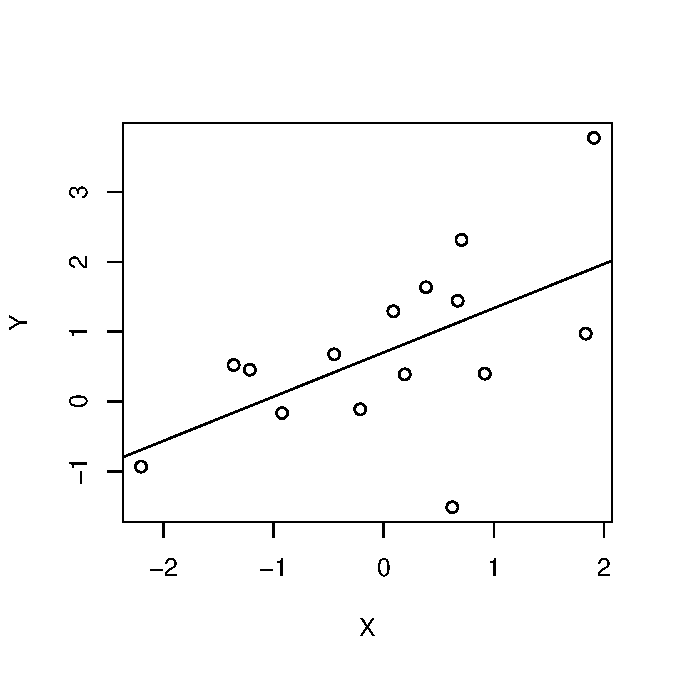
\includegraphics[width=.6\linewidth]{figure/beamer-lm-plot-1} 

}



\end{knitrout}
\end{frame}


\begin{frame}[fragile]
  \frametitle{One-way ANOVA}

\begin{knitrout}\footnotesize
\definecolor{shadecolor}{rgb}{0.969, 0.969, 0.969}\color{fgcolor}\begin{kframe}
\begin{alltt}
\hlstd{Z} \hlkwb{<-} \hlkwd{rnorm}\hlstd{(}\hlnum{10}\hlstd{)}
\hlstd{XYZ} \hlkwb{<-} \hlkwd{c}\hlstd{(X, Y, Z)}
\hlstd{Grp3} \hlkwb{<-} \hlkwd{factor}\hlstd{(}\hlkwd{c}\hlstd{(}\hlkwd{rep}\hlstd{(}\hlstr{"A"}\hlstd{,} \hlkwd{length}\hlstd{(X)),} \hlkwd{rep}\hlstd{(}\hlstr{"B"}\hlstd{,} \hlkwd{length}\hlstd{(Y)),}
                 \hlkwd{rep}\hlstd{(}\hlstr{"C"}\hlstd{,} \hlkwd{length}\hlstd{(Z))))}

\hlcom{## one-way ANOVA F-test}
\hlkwd{anova}\hlstd{(}\hlkwd{lm}\hlstd{(XYZ} \hlopt{~} \hlstd{Grp3))}
\hlcom{## Function aov() is a shortcut}
\hlkwd{summary}\hlstd{(}\hlkwd{aov}\hlstd{(XYZ} \hlopt{~} \hlstd{Grp3))}

\hlcom{# Kruskal-Wallis test (nonparametric)}
\hlkwd{kruskal.test}\hlstd{(XYZ, Grp3)}
\end{alltt}
\end{kframe}
\end{knitrout}
\end{frame}

\begin{frame}[fragile]
\begin{knitrout}\footnotesize
\definecolor{shadecolor}{rgb}{0.969, 0.969, 0.969}\color{fgcolor}\begin{kframe}
\begin{alltt}
\hlkwd{boxplot}\hlstd{(XYZ}\hlopt{~}\hlstd{Grp3,} \hlkwc{outpch} \hlstd{=} \hlnum{NA}\hlstd{,} \hlkwc{xlab}\hlstd{=}\hlstr{""}\hlstd{,} \hlkwc{ylab}\hlstd{=}\hlstr{"Value"}\hlstd{)}
\hlkwd{stripchart}\hlstd{(XYZ} \hlopt{~} \hlstd{Grp3,} \hlkwc{vertical}\hlstd{=}\hlnum{TRUE}\hlstd{,} \hlkwc{method}\hlstd{=}\hlstr{"jitter"}\hlstd{,}
           \hlkwc{add}\hlstd{=}\hlnum{TRUE}\hlstd{,} \hlkwc{pch}\hlstd{=}\hlnum{1}\hlstd{)}
\end{alltt}
\end{kframe}

{\centering 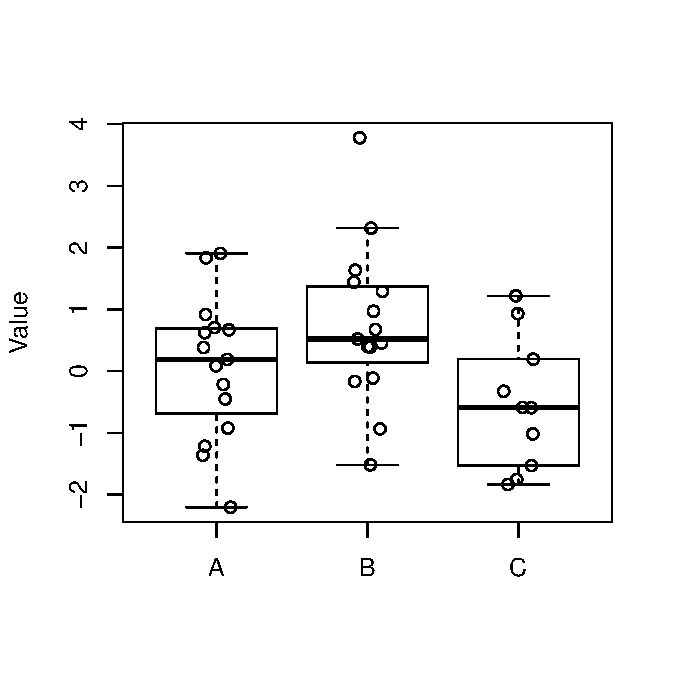
\includegraphics[width=.48\linewidth]{figure/beamer-one-anova-plot-1} 

}



\end{knitrout}
\end{frame}

\begin{frame}{Post-hoc analysis}
  \begin{itemize}
  \item More than often, we want to know which pairwise group
    comparison is significant.
  \item Proper way: 1. Test for overall significant. 2. Apply a
    suitable \textit{post hoc} analysis which controls the overall
    type I error.
  \item Methods: Tukey's \textit{post-hoc} analysis procedure for parametric test; 
  \item Common mistakes: 1. Pairwise $t$-test without adjustment.
  \end{itemize}
\end{frame}

\begin{frame}[fragile]{Post-hoc analysis example}

\begin{knitrout}\footnotesize
\definecolor{shadecolor}{rgb}{0.969, 0.969, 0.969}\color{fgcolor}\begin{kframe}
\begin{alltt}
\hlcom{## Tukey's procedure. Good for parametric test.}
\hlkwd{TukeyHSD}\hlstd{(}\hlkwd{aov}\hlstd{(XYZ} \hlopt{~} \hlstd{Grp3))}

\hlcom{## Dunn's test. Good for nonparametric test.}
\hlcom{# install.packages("dunn.test")}
\hlkwd{library}\hlstd{(}\hlstr{"dunn.test"}\hlstd{)}
\hlcom{## Here method="hs" means Holm-Sidak adjustment}
\hlkwd{dunn.test}\hlstd{(XYZ, Grp3,} \hlkwc{method}\hlstd{=}\hlstr{"hs"}\hlstd{)}
\end{alltt}
\end{kframe}
\end{knitrout}
\end{frame}

\begin{frame}{Repeated measures ANOVA}
  \begin{itemize}
  \item Imaging that you are observing data collected from 10 subjects
    (5 girls and 5 boys) at three time points: Day 0, 1, and 2.
  \item You want to test whether there is a significant Day effect or
    a Gender effect.
  \item Ordinary regression or one-way ANOVA is not appropriate due to
    correlation between errors.
  \item Solution: Repeated measures ANOVA and its nonparametric
    counterpart, Friedman's test.
  \end{itemize}
\end{frame}

\begin{frame}[fragile]{Repeated measures ANOVA example (I)}
\begin{knitrout}\footnotesize
\definecolor{shadecolor}{rgb}{0.969, 0.969, 0.969}\color{fgcolor}\begin{kframe}
\begin{alltt}
\hlcom{## generate some longitudinal data}
\hlstd{Gender} \hlkwb{<-} \hlkwd{rep}\hlstd{(}\hlkwd{c}\hlstd{(}\hlstr{"Female"}\hlstd{,} \hlstr{"Male"}\hlstd{),} \hlkwc{each}\hlstd{=}\hlnum{5}\hlstd{)}
\hlstd{Day0} \hlkwb{<-} \hlkwd{rnorm}\hlstd{(}\hlnum{10}\hlstd{)} \hlopt{+} \hlkwd{ifelse}\hlstd{(Gender}\hlopt{==}\hlstr{"Female"}\hlstd{,} \hlnum{3}\hlstd{,} \hlnum{0}\hlstd{)}
\hlstd{Day1} \hlkwb{<-} \hlstd{Day0} \hlopt{+} \hlkwd{ifelse}\hlstd{(Gender}\hlopt{==}\hlstr{"Female"}\hlstd{,} \hlnum{0}\hlstd{,} \hlnum{1}\hlstd{)} \hlopt{+} \hlkwd{rnorm}\hlstd{(}\hlnum{10}\hlstd{)}
\hlstd{Day2} \hlkwb{<-} \hlstd{Day1} \hlopt{+} \hlkwd{ifelse}\hlstd{(Gender}\hlopt{==}\hlstr{"Female"}\hlstd{,} \hlnum{0}\hlstd{,} \hlnum{1}\hlstd{)} \hlopt{+} \hlkwd{rnorm}\hlstd{(}\hlnum{10}\hlstd{)}
\hlcom{## Subject names }
\hlstd{SN} \hlkwb{<-} \hlkwd{paste}\hlstd{(}\hlstr{"sub"}\hlstd{,} \hlkwd{rep}\hlstd{(}\hlnum{1}\hlopt{:}\hlnum{10}\hlstd{,} \hlnum{3}\hlstd{),} \hlkwc{sep}\hlstd{=}\hlstr{""}\hlstd{)}
\hlcom{## combine them together}
\hlstd{mydata} \hlkwb{<-} \hlkwd{data.frame}\hlstd{(}\hlkwc{Y}\hlstd{=}\hlkwd{c}\hlstd{(Day0, Day1, Day2),}
                     \hlkwc{Day}\hlstd{=}\hlkwd{rep}\hlstd{(}\hlnum{0}\hlopt{:}\hlnum{2}\hlstd{,} \hlkwc{each}\hlstd{=}\hlnum{10}\hlstd{),}
                     \hlkwc{Gender}\hlstd{=}\hlkwd{rep}\hlstd{(Gender,} \hlnum{3}\hlstd{),}
                     \hlkwc{Subject}\hlstd{=SN)}
\end{alltt}
\end{kframe}
\end{knitrout}
\end{frame}

\begin{frame}[fragile]
\begin{knitrout}\footnotesize
\definecolor{shadecolor}{rgb}{0.969, 0.969, 0.969}\color{fgcolor}\begin{kframe}
\begin{alltt}
\hlkwd{plot}\hlstd{(Y}\hlopt{~}\hlstd{Day,} \hlkwc{data}\hlstd{=mydata,} \hlkwc{col}\hlstd{=}\hlkwd{ifelse}\hlstd{(Gender}\hlopt{==}\hlstr{"Female"}\hlstd{,} \hlstr{"red"}\hlstd{,} \hlstr{"black"}\hlstd{))}
\hlkwa{for} \hlstd{(i} \hlkwa{in} \hlnum{1}\hlopt{:}\hlnum{10}\hlstd{)\{}
    \hlkwd{lines}\hlstd{(Y}\hlopt{~}\hlstd{Day,} \hlkwc{data}\hlstd{=mydata[mydata[,} \hlstr{"Subject"}\hlstd{]}\hlopt{==}\hlkwd{paste}\hlstd{(}\hlstr{"sub"}\hlstd{, i,} \hlkwc{sep}\hlstd{=}\hlstr{""}\hlstd{),],}
          \hlkwc{col}\hlstd{=}\hlkwd{ifelse}\hlstd{(Gender}\hlopt{==}\hlstr{"Female"}\hlstd{,} \hlstr{"red"}\hlstd{,} \hlstr{"black"}\hlstd{))}
\hlstd{\}}
\end{alltt}
\end{kframe}

{\centering 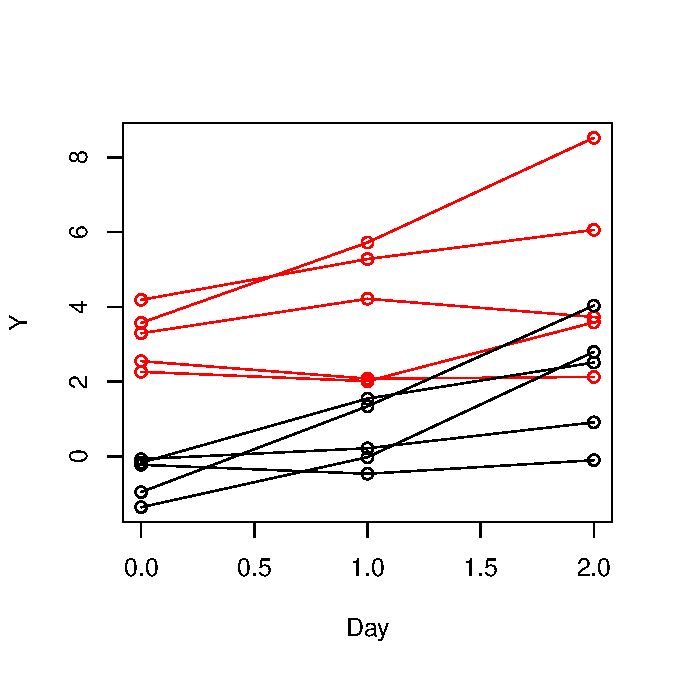
\includegraphics[width=.6\linewidth]{figure/beamer-rep-anova-plot-1} 

}



\end{knitrout}
\end{frame}

\begin{frame}[fragile]{Repeated measures ANOVA example (II)}
\begin{knitrout}\footnotesize
\definecolor{shadecolor}{rgb}{0.969, 0.969, 0.969}\color{fgcolor}\begin{kframe}
\begin{alltt}
\hlstd{mod2} \hlkwb{<-} \hlkwd{aov}\hlstd{(Y} \hlopt{~} \hlstd{Day} \hlopt{+} \hlkwd{Error}\hlstd{(Subject),} \hlkwc{data}\hlstd{=mydata)}
\hlkwd{summary}\hlstd{(mod2)}
\hlcom{## Two-way ANOVA with }
\hlstd{mod3} \hlkwb{<-} \hlkwd{aov}\hlstd{(Y} \hlopt{~} \hlstd{Day}\hlopt{+}\hlstd{Gender} \hlopt{+} \hlkwd{Error}\hlstd{(Subject),} \hlkwc{data}\hlstd{=mydata)}
\hlkwd{summary}\hlstd{(mod3)}

\hlcom{## Nonparametric version in simple case}
\hlkwd{friedman.test}\hlstd{(Y} \hlopt{~} \hlstd{Day} \hlopt{|} \hlstd{Subject,} \hlkwc{data}\hlstd{=mydata)}
\end{alltt}
\end{kframe}
\end{knitrout}
\end{frame}

\begin{frame}{Advanced linear regression and ANOVA techniques}
  \begin{itemize}
  \item A full-fledged linear mixed effect model can have many fixed
    and random factors, with the randomness encoded in both the
    intercept and slope terms. Package: \texttt{lme4}, function
    \texttt{lmer()}.
  \item Robust regression. \texttt{MASS}, \texttt{rlm()}.
  \item Ordinal regression.  \texttt{polr()}, \texttt{MASS}.
  \end{itemize}
\end{frame}

\section{Logistic Regression}
\label{sec:logistic-models}

\begin{frame}
\begin{itemize}
\item What if the response variable is \emph{binary}?
\item Answer: Logistic (or probit) regression.
  \begin{equation}
    \label{eq:logistic}
    \mathrm{logit} p := \log\frac{p}{1-p} = \mathbf{X}\bm{\beta}.
  \end{equation}
\item The above model is a special case of \emph{generalized linear
    model}, which also includes probit regression, Poisson regression,
  etc.
\item Function: \texttt{glm()}. 
\end{itemize}
\end{frame}

\begin{frame}[fragile]{Logistic regression}
\begin{knitrout}\footnotesize
\definecolor{shadecolor}{rgb}{0.969, 0.969, 0.969}\color{fgcolor}\begin{kframe}
\begin{alltt}
\hlstd{Smoke} \hlkwb{<-}  \hlkwd{c}\hlstd{(}\hlkwd{rep}\hlstd{(}\hlnum{0}\hlstd{,} \hlnum{10}\hlstd{),} \hlkwd{rep}\hlstd{(}\hlnum{1}\hlstd{,} \hlnum{10}\hlstd{),} \hlkwd{rep}\hlstd{(}\hlnum{2}\hlstd{,} \hlnum{10}\hlstd{),} \hlkwd{rep}\hlstd{(}\hlnum{3}\hlstd{,} \hlnum{10}\hlstd{))}
\hlstd{Cancer} \hlkwb{<-} \hlkwd{c}\hlstd{(}\hlkwd{rep}\hlstd{(}\hlnum{0}\hlstd{,} \hlnum{10}\hlstd{),} \hlkwd{rbinom}\hlstd{(}\hlnum{10}\hlstd{,} \hlnum{1}\hlstd{,} \hlnum{.3}\hlstd{),} \hlkwd{rbinom}\hlstd{(}\hlnum{10}\hlstd{,} \hlnum{1}\hlstd{,} \hlnum{.5}\hlstd{),} \hlkwd{rbinom}\hlstd{(}\hlnum{10}\hlstd{,} \hlnum{1}\hlstd{,} \hlnum{.8}\hlstd{))}
\hlstd{mod6} \hlkwb{<-} \hlkwd{glm}\hlstd{(Cancer} \hlopt{~} \hlstd{Smoke,} \hlkwc{family}\hlstd{=}\hlkwd{binomial}\hlstd{(}\hlkwc{link}\hlstd{=logit))}
\hlkwd{summary}\hlstd{(mod6)}
\end{alltt}
\end{kframe}
\end{knitrout}
\end{frame}

\begin{frame}{Other advanced regression models}
\begin{itemize}
\item Predicting expected rates of counting data in Poisson
  regression. Again \texttt{glm()}, with link function set to Poisson.
\item GLMs can also have random effect. Use \texttt{glmer()} from the
  \texttt{lme4} package.
\item Nonparametric regression, additive model, etc.
\end{itemize}
\end{frame}

\section{Introduction to categorical data analysis}
\label{sec:categ-data-analys}

\begin{frame}{$p\times q$ Contingency table}
  \begin{itemize}
  \item The association between smoking (as a binary variable) and
    lung cancer.
  \item Once summarized, it is a $2\times 2$ table.
  \item Suitable statistical test: $\chi^{2}$-test (Chi-square test,
    an approximate parametric test) and Fisher's exact test
    (nonparametric).
  \end{itemize}
\end{frame}

\begin{frame}[fragile]{Example of $2\times 2$ Contingency table}
\begin{knitrout}\footnotesize
\definecolor{shadecolor}{rgb}{0.969, 0.969, 0.969}\color{fgcolor}\begin{kframe}
\begin{alltt}
\hlstd{Smoke.binary} \hlkwb{<-} \hlkwd{ifelse}\hlstd{(Smoke}\hlopt{==}\hlnum{0}\hlstd{,} \hlnum{0}\hlstd{,} \hlnum{1}\hlstd{)}
\hlstd{ctab1} \hlkwb{<-} \hlkwd{table}\hlstd{(Smoke.binary, Cancer)}
\hlstd{ctab1}
\hlstd{ctab2} \hlkwb{<-} \hlkwd{table}\hlstd{(Smoke, Cancer)}        \hlcom{#4x2 table}
\hlkwd{chisq.test}\hlstd{(ctab1)}
\end{alltt}


{\ttfamily\noindent\color{warningcolor}{\#\# Warning in chisq.test(ctab1): Chi-squared approximation may be incorrect}}\begin{alltt}
\hlkwd{fisher.test}\hlstd{(ctab1)}
\hlkwd{chisq.test}\hlstd{(ctab2)}
\end{alltt}


{\ttfamily\noindent\color{warningcolor}{\#\# Warning in chisq.test(ctab2): Chi-squared approximation may be incorrect}}\begin{alltt}
\hlkwd{fisher.test}\hlstd{(ctab2)}
\end{alltt}
\end{kframe}
\end{knitrout}

\end{frame}

\begin{frame}{Generalized Cochran-Mantel-Haenszel Tests}
  \begin{itemize}
  \item Cochran-Mantel-Haenszel test (function
    \texttt{mantelhaen.test()}) can test $p\times q$ table observed at
    several different timen points.
  \item Package \texttt{vcdExtra} has a function \texttt{CMHtest()}
    that can test the association between two \emph{ordinal} factors,
    possibly observed at several time points.
  \end{itemize}
\end{frame}

\section{Other topics}
\label{sec:other-topics}

\begin{frame}
  \frametitle{Linear discriminant analysis}
  \begin{itemize}
  \item A predictive model that finds the best \emph{linear}
    separation between two classes.
  \item It is a form of \emph{supervised learning} and is an
    alternative to logistic regression.
  \item \texttt{lda()} of \texttt{MASS}.
  \end{itemize}
\end{frame}

\begin{frame}[fragile]{LDA Example}
\begin{knitrout}\footnotesize
\definecolor{shadecolor}{rgb}{0.969, 0.969, 0.969}\color{fgcolor}\begin{kframe}
\begin{alltt}
\hlcom{## Group A.}
\hlstd{A} \hlkwb{<-} \hlkwd{data.frame}\hlstd{(}\hlkwc{X}\hlstd{=}\hlkwd{rnorm}\hlstd{(}\hlnum{30}\hlstd{,} \hlnum{0}\hlstd{,} \hlnum{1}\hlstd{),} \hlkwc{Y}\hlstd{=}\hlkwd{rnorm}\hlstd{(}\hlnum{30}\hlstd{,} \hlnum{0}\hlstd{,} \hlnum{2}\hlstd{))}
\hlstd{B} \hlkwb{<-} \hlkwd{data.frame}\hlstd{(}\hlkwc{X}\hlstd{=}\hlkwd{rnorm}\hlstd{(}\hlnum{20}\hlstd{,} \hlnum{2}\hlstd{,} \hlnum{1}\hlstd{),} \hlkwc{Y}\hlstd{=}\hlkwd{rnorm}\hlstd{(}\hlnum{20}\hlstd{,} \hlnum{3}\hlstd{,} \hlnum{2}\hlstd{))}
\hlstd{mydata2} \hlkwb{<-} \hlkwd{cbind}\hlstd{(}\hlkwd{rbind}\hlstd{(A, B),}
                 \hlkwc{Grp}\hlstd{=}\hlkwd{c}\hlstd{(}\hlkwd{rep}\hlstd{(}\hlstr{"A"}\hlstd{,} \hlnum{30}\hlstd{),} \hlkwd{rep}\hlstd{(}\hlstr{"B"}\hlstd{,} \hlnum{20}\hlstd{)))}
\hlkwd{library}\hlstd{(MASS)}
\hlcom{## attach() makes objects in a data.frame visible}
\hlcom{### at the top-level}
\hlkwd{rm}\hlstd{(}\hlkwc{list}\hlstd{=}\hlkwd{c}\hlstd{(}\hlstr{"X"}\hlstd{,}\hlstr{"Y"}\hlstd{,}\hlstr{"Grp"}\hlstd{));} \hlkwd{attach}\hlstd{(mydata2)}
\hlstd{mod7} \hlkwb{<-} \hlkwd{lda}\hlstd{(Grp}\hlopt{~}\hlstd{X}\hlopt{+}\hlstd{Y)}
\hlstd{ss1} \hlkwb{<-} \hlstd{mod7}\hlopt{$}\hlstd{scaling}            \hlcom{# discriminant function coefs}
\hlstd{ss1}
\hlstd{cc1} \hlkwb{<-} \hlkwd{mean}\hlstd{(ss1[}\hlnum{1}\hlstd{]} \hlopt{*} \hlstd{X} \hlopt{+} \hlstd{ss1[}\hlnum{2}\hlstd{]} \hlopt{*} \hlstd{Y)} \hlcom{#cutoff point}
\hlstd{cc1}
\hlkwd{detach}\hlstd{(mydata2)}
\end{alltt}
\end{kframe}
\end{knitrout}
\end{frame}

\begin{frame}[fragile]
\begin{knitrout}\footnotesize
\definecolor{shadecolor}{rgb}{0.969, 0.969, 0.969}\color{fgcolor}\begin{kframe}
\begin{alltt}
\hlkwd{with}\hlstd{(mydata2,} \hlkwd{plot}\hlstd{(X, Y,} \hlkwc{pch}\hlstd{=}\hlkwd{ifelse}\hlstd{(Grp}\hlopt{==}\hlstr{"A"}\hlstd{,} \hlnum{1}\hlstd{,} \hlnum{19}\hlstd{)))}
\hlkwd{abline}\hlstd{(cc1}\hlopt{/}\hlstd{ss1[}\hlnum{2}\hlstd{],} \hlopt{-}\hlstd{ss1[}\hlnum{1}\hlstd{]}\hlopt{/}\hlstd{ss1[}\hlnum{2}\hlstd{],} \hlkwc{lty}\hlstd{=}\hlnum{2}\hlstd{)}
\hlkwd{legend}\hlstd{(}\hlstr{"topright"}\hlstd{,}
       \hlkwc{legend}\hlstd{=}\hlkwd{c}\hlstd{(}\hlstr{"A"}\hlstd{,} \hlstr{"B"}\hlstd{),}
       \hlkwc{pch}\hlstd{=}\hlkwd{c}\hlstd{(}\hlnum{1}\hlstd{,}\hlnum{19}\hlstd{))}
\end{alltt}
\end{kframe}

{\centering 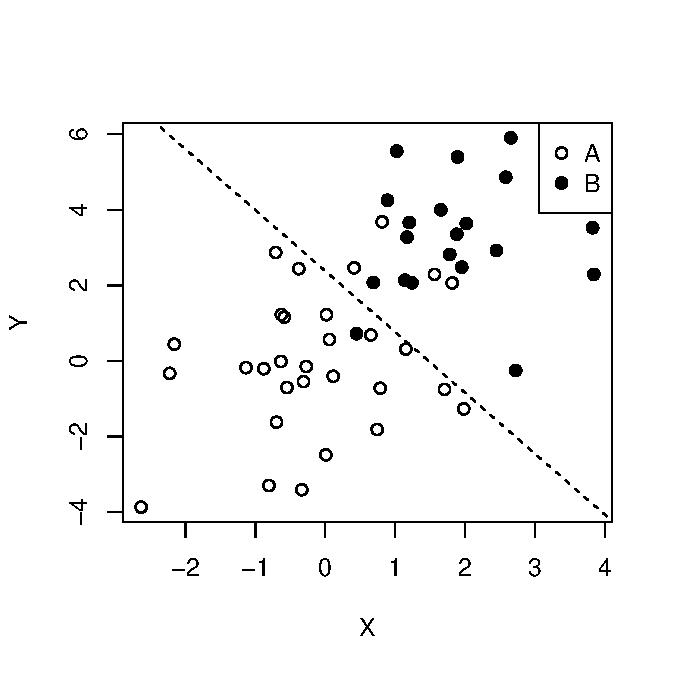
\includegraphics[width=.6\linewidth]{figure/beamer-lda-plot-1} 

}



\end{knitrout}
  
\end{frame}

\begin{frame}[fragile]
  \frametitle{ROC Curves}
  \begin{itemize}
  \item Receiver operating characteristic (ROC) curve.  Package: \texttt{ROCR}
    package.
  \item Trade-off between type I and type II errors.
  \end{itemize}
  {\centering 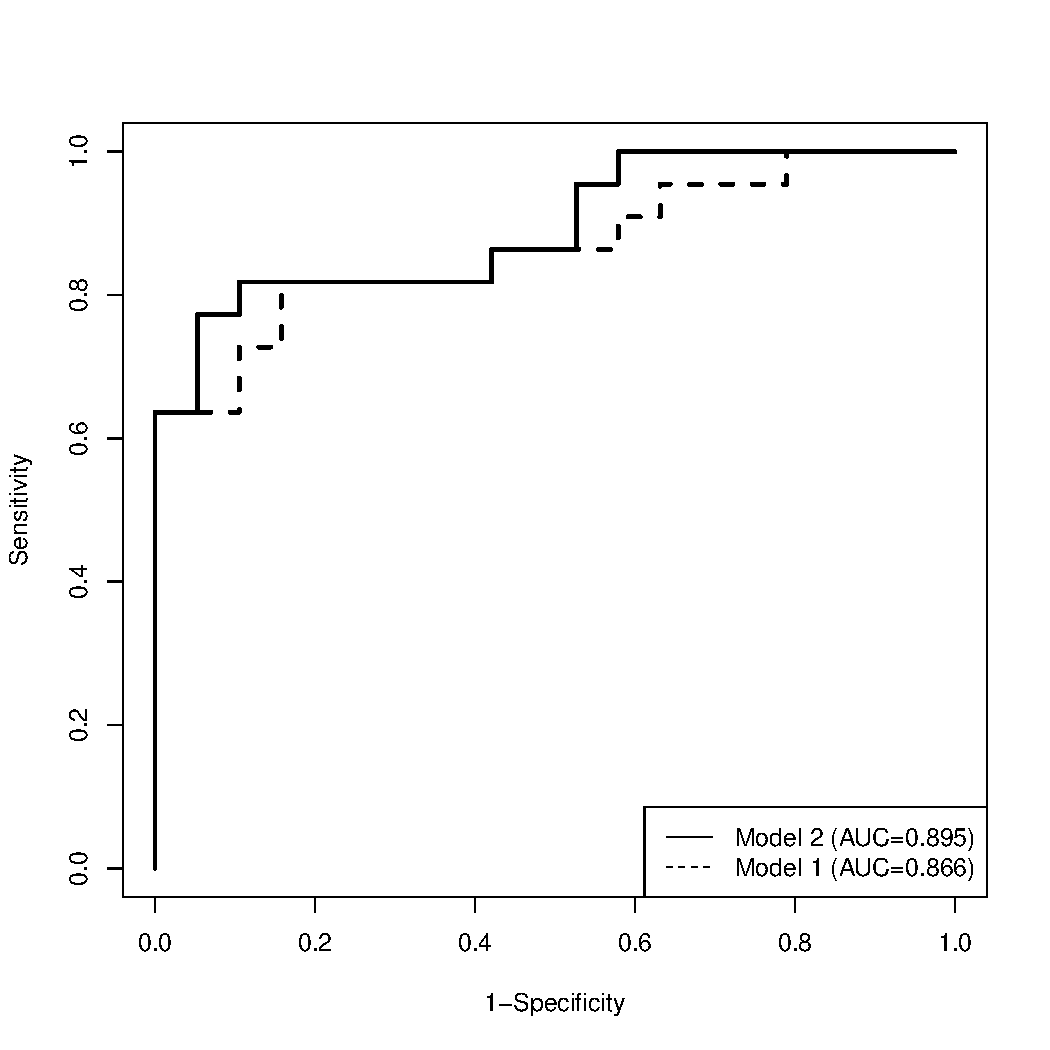
\includegraphics[width=.48\linewidth]{roc}}
\end{frame}

\begin{frame}{Survival Analysis}
  \begin{itemize}
  \item Assume that we want to establish the association between some
    clinical covariates and the \emph{survival time} of patients.
  \item What if many subjects survived the trial?
  \item Censored data shouldn't be treated as ``missing'' or
    ``truncated''.
  \item One of the most popular model: Cox proportional hazards model.
    Function: \texttt{coxph()} from the \texttt{survival} package.
  \end{itemize}
\end{frame}

\begin{frame}
  \frametitle{Cluster analysis}
  \begin{itemize}
  \item Hierarchical cluster analysis.
  \item Distance-based methods. \texttt{kmeans()}, \texttt{skmeans()}.
  \item Model-based approaches. Package\texttt{Mclust} includes
    several most popular models.
  \item Specialized methods. Time course data etc.
  \end{itemize}
\end{frame}

\begin{frame}
  \frametitle{Power analysis}
  \begin{itemize}
  \item What you need: A comparable study from which you can find:
    $n_{1}$, $n_{2}$, $d= \dfrac{\left|\mu_{1}-
        \mu_{2}\right|}{\sigma_{\mathrm{pool}}}$.
  \item Justify that the proposed study is comparable to that prior study.  
  \item Package: \texttt{pwr}, \texttt{pwr.t2n.test()},
    \texttt{pwr.anova.test()} etc.
  \end{itemize}
\end{frame}

\begin{frame}
  \frametitle{Other topics}
  \begin{itemize}
  \item Financial engineering, time series data analysis, machine
    learning, Bayesian inference, image analysis, high-performance
    computing, etc.
  \item Differential equation solvers, inverse problem (will be
    discussed in Profs. Wu and Miao's class).
  \item Bioinformatics related topics will be discussed in detail on
    6/3.
  \end{itemize}
\end{frame}

\begin{frame}[allowframebreaks]{Bibliography}
  \bibliographystyle{amsplain}
  \bibliography{xing}
\end{frame}


%%% Local Variables:
%%% mode: latex
%%% TeX-master: "presentation"
%%% TeX-PDF-mode: t
%%% End:
